% questions.tex —— 2012 年·重庆卷·文科 · 题目内容片段（无答案）
% 由 tools/generate_projects.py 依来源总账自 2012/2012_数学真题_重庆文_试题.md 生成，勿手改（改源 MD 后重跑）

\gkpart{一、选择题}

\begin{question}
\gkti{1}命题“若 $p$ 则 $q$”的逆命题是\mbox{（　　）}

（A）若 $q$ 则 $p$；（B）若 $\neg p$ 则 $\neg q$；（C）若 $\neg q$ 则 $\neg p$；（D）若 $p$ 则 $\neg q$。

\end{question}
\begin{question}
\gkti{2}不等式 $\dfrac{x-1}{x+2}<0$ 的解集为\mbox{（　　）}

（A）$(1,+\infty)$；（B）$(-\infty,-2)$；（C）$(-2,1)$；（D）$(-\infty,-2)\cup(1,+\infty)$。

\end{question}
\begin{question}
\gkti{3}设 $A$，$B$ 为直线 $y=x$ 与圆 $x^2+y^2=1$ 的两个交点，则 $|AB|=$\mbox{（　　）}

（A）$1$；（B）$\sqrt2$；（C）$\sqrt3$；（D）$2$。

\end{question}
\begin{question}
\gkti{4}$(1-3x)^5$ 的展开式中 $x^3$ 的系数为\mbox{（　　）}

（A）$-270$；（B）$-90$；（C）$90$；（D）$270$。

\end{question}
\begin{question}
\gkti{5}$\dfrac{\sin47^\circ-\sin17^\circ\cos30^\circ}{\cos17^\circ}=$\mbox{（　　）}

（A）$-\dfrac{\sqrt3}2$；（B）$-\dfrac12$；（C）$\dfrac12$；（D）$\dfrac{\sqrt3}2$。

\end{question}
\begin{question}
\gkti{6}设 $x\in\mathbf R$，向量 $\boldsymbol a=(x,1)$，$\boldsymbol b=(1,-2)$，且 $\boldsymbol a\perp\boldsymbol b$，则 $|\boldsymbol a+\boldsymbol b|=$\mbox{（　　）}

（A）$\sqrt5$；（B）$\sqrt{10}$；（C）$2\sqrt5$；（D）$10$。

\end{question}
\begin{question}
\gkti{7}已知 $a=\log_23+\log_2\sqrt3$，$b=\log_29-\log_2\sqrt3$，$c=\log_32$，则 $a$，$b$，$c$ 的大小关系是\mbox{（　　）}

（A）$a=b<c$；（B）$a=b>c$；（C）$a<b<c$；（D）$a>b>c$。

\Needspace{0.4\textheight}
\end{question}
\begin{question}
\gkti{8}设函数 $f(x)$ 在 $\mathbf R$ 上可导，其导函数为 $f'(x)$，且函数 $f(x)$ 在 $x=-2$ 处取得极小值，则函数 $y=xf'(x)$ 的图象可能是\mbox{（　　）}
\nopagebreak[4]
\begin{center}% 2012 年重庆卷文科第 8 题：y=xf'(x) 的四个图象选项。
% 来源 PDF：普通高考/2012/2012重庆文.pdf，第 1 页（印面 723）第 2 栏。
% 选项 (B) 为零点 x=-2 与 x=0、在 (-2,0) 内为负、两侧为正的图象，即正确答案。
\begin{tikzpicture}[scale=0.78, semithick, >=Stealth, font=\small]
  \foreach \dx/\dy/\lab in {0/0/{(A)}, 5.4/0/{(B)}, 0/-5.2/{(C)}, 5.4/-5.2/{(D)}} {
    \begin{scope}[shift={(\dx,\dy)}]
      \clip (-2.3,-1.9) rectangle (2.3,1.9);
      \draw[->] (-2.4,0) -- (2.4,0) node[right] {$x$};
      \draw[->] (0,-2.0) -- (0,2.0) node[above] {$y$};
      \node[below left] at (0,0) {\scriptsize $O$};
    \end{scope}
    \node[below] at (\dx,\dy-2.35) {\lab};
  }
  % (A)
  \begin{scope}[shift={(0,0)}]
    \clip (-2.3,-1.9) rectangle (2.3,1.9);
    \draw[smooth, domain=-2.3:1.2] plot (\x, {-0.6*\x*(\x+2.4)});
  \end{scope}
  % (B)
  \begin{scope}[shift={(5.4,0)}]
    \clip (-2.3,-1.9) rectangle (2.3,1.9);
    \draw[smooth, domain=-2.3:1.4] plot (\x, {0.55*\x*(\x+2)});
    \node[below] at (-2,-0.05) {\scriptsize $-2$};
  \end{scope}
  % (C)
  \begin{scope}[shift={(0,-5.2)}]
    \clip (-2.3,-1.9) rectangle (2.3,1.9);
    \draw[smooth, domain=-2.3:2.0] plot (\x, {0.8*\x});
  \end{scope}
  % (D)
  \begin{scope}[shift={(5.4,-5.2)}]
    \clip (-2.3,-1.9) rectangle (2.3,1.9);
    \draw[smooth, domain=-2.3:1.4] plot (\x, {-0.55*\x*(\x+2)});
    \node[below] at (-2,-0.05) {\scriptsize $-2$};
  \end{scope}
\end{tikzpicture}
\end{center}
\nopagebreak[4]
\end{question}
\begin{question}
\gkti{9}设四面体的六条棱的长分别为 $1$，$1$，$1$，$1$，$\sqrt2$ 和 $a$，且长为 $a$ 的棱与长为 $\sqrt2$ 的棱异面，则 $a$ 的取值范围是\mbox{（　　）}

（A）$\left(0,\sqrt2\right)$；（B）$\left(0,\sqrt3\right)$；（C）$\left(1,\sqrt2\right)$；（D）$\left(1,\sqrt3\right)$。

\end{question}
\begin{question}
\gkti{10}设函数 $f(x)=x^2-4x+3$，$g(x)=3^x-2$，集合 $M=\{x\in\mathbf R\mid f(g(x))>0\}$，$N=\{x\in\mathbf R\mid g(x)<2\}$，则 $M\cap N$ 为\mbox{（　　）}

（A）$(1,+\infty)$；（B）$(0,1)$；（C）$(-1,1)$；（D）$(-\infty,1)$。

\end{question}
\gkpart{二、填空题}

\begin{question}
\gkti{11}首项为 $1$，公比为 $2$ 的等比数列的前 $4$ 项和 $S_4=$\gkblank{}。

\end{question}
\begin{question}
\gkti{12}若 $f(x)=(x+a)(x-4)$ 为偶函数，则实数 $a=$\gkblank{}。

\end{question}
\begin{question}
\gkti{13}设 $\triangle ABC$ 的内角 $A$，$B$，$C$ 的对边分别为 $a$，$b$，$c$，且 $a=1$，$b=2$，$\cos C=\dfrac14$，则 $\sin B=$\gkblank{}。

\end{question}
\begin{question}
\gkti{14}设 $P$ 为直线 $y=\dfrac b{3a}x$ 与双曲线 $\dfrac{x^2}{a^2}-\dfrac{y^2}{b^2}=1$（$a>0$，$b>0$）左支的交点，$F_1$ 是左焦点，$PF_1$ 垂直于 $x$ 轴，则双曲线的离心率 $e=$\gkblank{}。

\end{question}
\begin{question}
\gkti{15}某艺校在一天的 $6$ 节课中随机安排语文、数学、外语三门文化课和其他三门艺术课各 $1$ 节，则在课表上的相邻两节文化课之间至少间隔 $1$ 节艺术课的概率为\gkblank{}。（用数字作答）

\end{question}
\gkpart{三、解答题}

\begin{question}
\gkti{16}已知 $\{a_n\}$ 为等差数列，且 $a_1+a_3=8$，$a_2+a_4=12$。

（1） 求 $\{a_n\}$ 的通项公式；

（2） 记 $\{a_n\}$ 的前 $n$ 项和为 $S_n$，若 $a_1$，$a_k$，$a_{k+2}$ 成等比数列，求正整数 $k$ 的值。

\end{question}
\begin{question}
\gkti{17}已知函数 $f(x)=ax^3+bx+c$ 在点 $x=2$ 处取得极值 $c-16$。

（1） 求 $a$，$b$ 的值；

（2） 若 $f(x)$ 有极大值 $28$，求 $f(x)$ 在 $[-3,3]$ 上的最小值。

\end{question}
\begin{question}
\gkti{18}甲、乙两人轮流投篮，每人每次投一球。约定甲先投且先投中者获胜，一直到有人获胜或每人都已投球 $3$ 次时投篮结束。设甲每次投篮投中的概率为 $\dfrac13$，乙每次投篮投中的概率为 $\dfrac12$，且各次投篮互不影响。

（1） 求乙获胜的概率；

（2） 求投篮结束时乙只投了 $2$ 个球的概率。

\end{question}
\begin{question}
\gkti{19}设函数 $f(x)=A\sin(\omega x+\varphi)$（其中 $A>0$，$\omega>0$，$-\pi<\varphi\leqslant\pi$）在 $x=\dfrac\pi6$ 处取得最大值 $2$，其图象与 $x$ 轴的相邻两个交点的距离为 $\dfrac\pi2$。

（1） 求 $f(x)$ 的解析式；

（2） 求函数 $g(x)=\dfrac{6\cos^4x-\sin^2x-1}{f\left(x+\dfrac\pi6\right)}$ 的值域。

\Needspace{0.4\textheight}
\end{question}
\begin{question}
\gkti{20}如图，在直三棱柱 $ABC-A_1B_1C_1$ 中，$AB=4$，$AC=BC=3$，$D$ 为 $AB$ 的中点。

（1） 求异面直线 $CC_1$ 和 $AB$ 的距离；

（2） 若 $AB_1\perp A_1C$，求二面角 $A_1-CD-B_1$ 的平面角的余弦值。
\nopagebreak[4]
\begin{center}% 2012 年重庆卷文科第 20 题：直三棱柱 ABC-A1B1C1，D 为 AB 中点。
% 来源 PDF：普通高考/2012/2012重庆文.pdf，第 2 页（印面 724）第 2 栏。
% 投影：screen(x,y,z) = (x + 0.45y, 0.55y + 0.75z)，取 AB=4、CD=√5、高 2√2。
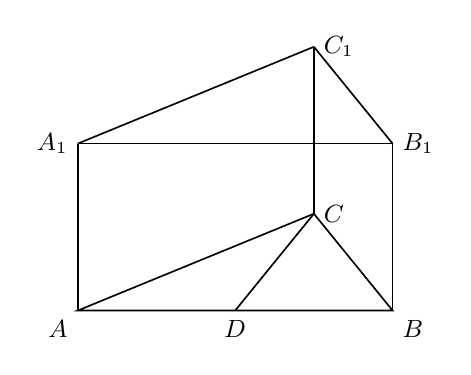
\begin{tikzpicture}[semithick, font=\small]
  \coordinate (A)  at (-2,0);
  \coordinate (B)  at (2,0);
  \coordinate (C)  at (1.0,1.23);
  \coordinate (D)  at (0,0);
  \coordinate (A1) at (-2,2.12);
  \coordinate (B1) at (2,2.12);
  \coordinate (C1) at (1.0,3.35);
  \draw (A) -- (B) -- (C) -- cycle;
  \draw (A) -- (A1);
  \draw (B) -- (B1);
  \draw (C) -- (C1);
  \draw (A1) -- (B1);
  \draw (B1) -- (C1);
  \draw (A1) -- (C1);
  \draw (C) -- (D);
  \node[below left] at (A) {$A$};
  \node[below right] at (B) {$B$};
  \node[right] at (C) {$C$};
  \node[below] at (D) {$D$};
  \node[left] at (A1) {$A_1$};
  \node[right] at (B1) {$B_1$};
  \node[right] at (C1) {$C_1$};
\end{tikzpicture}
\end{center}
\nopagebreak[4]
\Needspace{0.4\textheight}
\end{question}
\begin{question}
\gkti{21}如图，设椭圆的中心为原点 $O$，长轴在 $x$ 轴上，上顶点为 $A$，左、右焦点分别为 $F_1$，$F_2$，线段 $OF_1$，$OF_2$ 的中点分别为 $B_1$，$B_2$，且 $\triangle AB_1B_2$ 是面积为 $4$ 的直角三角形。

（1） 求该椭圆的离心率和标准方程；

（2） 过 $B_1$ 作直线交椭圆于 $P$，$Q$ 两点，使 $PB_2\perp QB_2$，求 $\triangle PB_2Q$ 的面积。
\nopagebreak[4]
\begin{center}% 2012 年重庆卷文科第 21 题：椭圆上顶点 A、焦点 F1、F2 与 OF 中点 B1、B2。
% 来源 PDF：普通高考/2012/2012重庆文.pdf，第 2 页（印面 724）第 3 栏。
% 按 (1) 的结果 a=2√5、b=2、c=4 作图：A(0,2)，B1(-2,0)，B2(2,0)。
\begin{tikzpicture}[scale=0.62, semithick, >=Stealth, font=\small]
  \draw (0,0) ellipse (4.472 and 2);
  \draw[->] (-5.6,0) -- (5.8,0) node[right] {$x$};
  \draw[->] (0,-3.0) -- (0,3.2) node[above] {$y$};
  \coordinate (A) at (0,2);
  \coordinate (F1) at (-4,0);
  \coordinate (F2) at (4,0);
  \coordinate (B1) at (-2,0);
  \coordinate (B2) at (2,0);
  \fill (A) circle (2.4pt);
  \fill (F1) circle (2.4pt);
  \fill (F2) circle (2.4pt);
  \fill (B1) circle (2.4pt);
  \fill (B2) circle (2.4pt);
  \node[above] at (A) {$A$};
  \node[below left] at (F1) {$F_1$};
  \node[below right] at (F2) {$F_2$};
  \node[below left] at (B1) {$B_1$};
  \node[below right] at (B2) {$B_2$};
  \node[below left] at (0,0) {$O$};
  \draw (A) -- (B1) -- (B2) -- cycle;
\end{tikzpicture}
\end{center}
\nopagebreak[4]

\end{question}